\newpage
\section{La Loi Log-Normale}

\subsection{Introduction et Définition}

Après la loi normale, qui modélise des phénomènes résultant de \textit{l'addition} de nombreux petits effets, nous abordons une loi qui modélise le \textit{produit} de nombreux petits facteurs.

\begin{definitionbox}[Loi Log-Normale]
Une variable aléatoire continue $Y$ suit une \textbf{loi log-normale} de paramètres $\mu$ et $\sigma^2$, notée $Y \sim \text{Log-}\mathcal{N}(\mu, \sigma^2)$, si son logarithme népérien $X = \ln(Y)$ suit une loi normale $\mathcal{N}(\mu, \sigma^2)$.

Puisque $\ln(Y)$ doit être un nombre réel, le support de $Y$ (l'ensemble des valeurs qu'elle peut prendre) est l'intervalle $(0, \infty)$.
\end{definitionbox}

\begin{remarquebox}[Interprétation Cruciale des Paramètres]
C'est le point le plus important (et le plus confus) de la loi log-normale :
\begin{itemize}
    \item $\mu$ \textbf{n'est PAS} l'espérance de $Y$.
    \item $\sigma^2$ \textbf{n'est PAS} la variance de $Y$.
\end{itemize}
Au lieu de cela, $\mu = E[\ln(Y)]$ et $\sigma^2 = \text{Var}(\ln(Y))$ sont l'espérance et la variance de la variable normale \textit{sous-jacente} (le log de $Y$).
\end{remarquebox}

\subsection{Intuition : Des Sommes aux Produits}

La loi log-normale peut sembler complexe, mais elle émerge naturellement de processus multiplicatifs, tout comme la loi normale émerge de processus additifs.

\begin{intuitionbox}[Du Multiplicatif à l'Additif (et retour)]
\textbf{1. Le Contraste (Additif $\to$ Normal)} :
La loi normale (via le Théorème Central Limite) décrit le résultat d'une \textbf{somme} de nombreux petits chocs aléatoires indépendants (comme les $\pm 1$ d'un jeu de pile ou face répété). Le résultat est symétrique autour d'une moyenne.
$$ S_n = X_1 + X_2 + \ldots + X_n \quad \xrightarrow{\text{TCL}} \quad \mathcal{N} $$

\textbf{2. Le Problème (Multiplicatif)} :
De nombreux phénomènes réels ne s'additionnent pas, ils se \textit{multiplient}.
\begin{itemize}
    \item \textbf{Finance :} Un capital $C$ évolue par des rendements en pourcentage. $C_T = C_0 \times (1+r_1) \times (1+r_2) \times \ldots \times (1+r_T)$.
    \item \textbf{Biologie :} La taille d'une population de bactéries est $P_t = P_0 \times F_1 \times F_2 \times \ldots \times F_t$, où $F_i$ est le facteur de croissance à l'étape $i$.
\end{itemize}
Nous voulons décrire la distribution d'un \textbf{produit} de facteurs aléatoires :
$$ Y = F_1 \times F_2 \times \ldots \times F_n $$

\textbf{3. L'Astuce (Le Logarithme)} :
Les produits sont difficiles à manipuler. L'astuce mathématique fondamentale est de prendre le logarithme, qui \textbf{transforme les produits en sommes} :
$$ \ln(Y) = \ln(F_1) + \ln(F_2) + \ldots + \ln(F_n) $$

\textbf{4. L'Apparition de la Loi Normale} :
Nous avons transformé notre problème ! La variable $\ln(Y)$ est maintenant une \textit{somme} de petits chocs aléatoires (les $\ln(F_i)$). D'après le Théorème Central Limite, si $n$ est grand, la distribution de cette \textit{somme} $\ln(Y)$ va converger vers une loi normale.
$$ \ln(Y) = X \sim \mathcal{N}(\mu, \sigma^2) $$
C'est l'origine du nom "log-normal" : le \textit{log} de la variable est \textit{normal}.

\textbf{5. Le Retour (L'Exponentielle)} :
Pour trouver la distribution de $Y$ (notre variable d'intérêt), il nous faut inverser l'opération du logarithme. Nous prenons l'exponentielle :
$$ Y = e^X \quad \text{où } X \sim \mathcal{N}(\mu, \sigma^2) $$
Cette transformation $x \mapsto e^x$ change radicalement la forme de la distribution.
\begin{itemize}
    \item La cloche symétrique de $X$ (qui peut être négative) est transformée.
    \item Puisque $e^x > 0$ pour tout $x$, la variable $Y$ est \textbf{strictement positive}.
    \item La partie gauche de la cloche (valeurs $x \to -\infty$) est \textbf{compressée} près de $0$ ($e^x \to 0$).
    \item La partie droite de la cloche (valeurs $x \to +\infty$) est \textbf{étirée} exponentiellement ($e^x \to \infty$).
\end{itemize}
Le résultat est une distribution \textbf{asymétrique à droite} (biaisée positivement), avec une longue queue vers les valeurs élevées.

\textbf{Conclusion :} La loi log-normale est la loi des \textbf{produits} de nombreux petits facteurs aléatoires. Elle modélise des grandeurs qui ne peuvent être négatives et qui ont une probabilité non négligeable d'atteindre des valeurs très grandes.
\end{intuitionbox}

\subsection{Fonction de Densité (PDF)}

On peut déduire la forme de la PDF log-normale en utilisant la méthode du changement de variable sur $Y = e^X$.

\begin{theorembox}[Fonction de Densité Log-Normale]
Si $Y \sim \text{Log-}\mathcal{N}(\mu, \sigma^2)$, sa fonction de densité de probabilité est donnée par :
$$ f_Y(y) = \frac{1}{y \sigma \sqrt{2\pi}} e^{ -\frac{(\ln(y) - \mu)^2}{2\sigma^2} } $$
pour tout $y > 0$.
\end{theorembox}

\begin{proofbox}[Dérivation par Changement de Variable]
Nous cherchons la densité $f_Y(y)$ de $Y = g(X) = e^X$, sachant que $X = g^{-1}(Y) = \ln(Y)$ a pour densité $f_X(x) = \phi\left(\frac{x-\mu}{\sigma}\right) \frac{1}{\sigma}$.
La formule de changement de variable est $f_Y(y) = f_X(g^{-1}(y)) \left| \frac{d(g^{-1}(y))}{dy} \right|$.
Ici, $x = g^{-1}(y) = \ln(y)$.
La dérivée est $\frac{dx}{dy} = \frac{1}{y}$. Puisque $y > 0$, on a $|\frac{1}{y}| = \frac{1}{y}$.
Substituons $x = \ln(y)$ dans la densité de $X$ et multiplions par la dérivée :
$$ f_Y(y) = f_X(\ln(y)) \cdot \frac{1}{y} $$
$$ f_Y(y) = \left[ \frac{1}{\sigma \sqrt{2\pi}} e^{ -\frac{1}{2} \left( \frac{\ln(y)-\mu}{\sigma} \right)^2 } \right] \cdot \frac{1}{y} $$
En réarrangeant, on obtient :
$$ f_Y(y) = \frac{1}{y \sigma \sqrt{2\pi}} e^{ -\frac{(\ln(y) - \mu)^2}{2\sigma^2} } $$
\end{proofbox}

\begin{intuitionbox}[Forme de la PDF]
La PDF log-normale confirme notre intuition :
\begin{itemize}
    \item Elle n'est définie que pour $y > 0$.
    \item Elle est fortement \textbf{asymétrique à droite}. Elle commence à $f_Y(0)=0$, monte rapidement vers un pic (le mode), puis redescend lentement, formant une longue "queue" vers les grandes valeurs.
    \item Le paramètre $\sigma$ (l'écart-type de $\ln Y$) contrôle \textbf{l'asymétrie} de $Y$. Un $\sigma$ plus grand rend la distribution plus étalée et plus asymétrique.
\end{itemize}

\tcblower
\centering
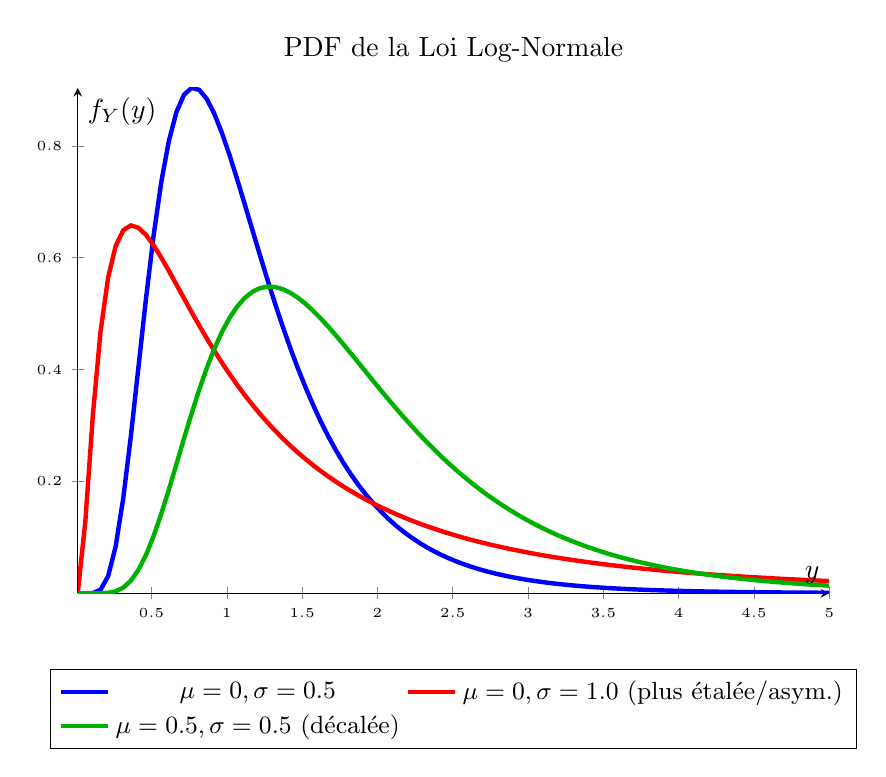
\begin{tikzpicture}
    \begin{axis}[
        title={PDF de la Loi Log-Normale},
        xlabel={$y$},
        ylabel={$f_Y(y)$},
        axis lines=middle,
        no markers,
        samples=100,
        domain=0.01:5, % Domaine > 0
        height=8cm,
        width=\linewidth-1cm,
        tick label style={font=\tiny},
        legend style={at={(0.5,-0.15)}, anchor=north, font=\small},
        legend columns=2
    ]
    % Log-N(0, 0.25) => mu=0, sigma=0.5
    \addplot [blue, ultra thick] {1/(x*0.5*sqrt(2*pi))*exp(-(ln(x)-0)^2/(2*0.5^2))};
    \addlegendentry{$\mu=0, \sigma=0.5$};
    % Log-N(0, 1) => mu=0, sigma=1
    \addplot [red, ultra thick] {1/(x*1*sqrt(2*pi))*exp(-(ln(x)-0)^2/(2*1^2))};
    \addlegendentry{$\mu=0, \sigma=1.0$ (plus étalée/asym.)};
    % Log-N(0.5, 0.25) => mu=0.5, sigma=0.5
    \addplot [green!70!black, ultra thick] {1/(x*0.5*sqrt(2*pi))*exp(-(ln(x)-0.5)^2/(2*0.5^2))};
    \addlegendentry{$\mu=0.5, \sigma=0.5$ (décalée)};
    \end{axis}
\end{tikzpicture}
\par\small\textit{Influence de $\mu$ (échelle) et $\sigma$ (forme/asymétrie) sur la PDF log-normale.}
\end{intuitionbox}

\subsection{Comment obtenir l’espérance d’une variable log-normale}

L’espérance d’une variable log-normale ne se calcule pas directement à partir de sa densité sans précaution, car la forme de cette densité rend l’intégrale peu intuitive. Heureusement, la définition même de la loi log-normale — via une transformation exponentielle d’une variable normale — fournit une voie élégante et puissante.

\begin{intuitionbox}[Stratégie de calcul : exploiter la variable sous-jacente]
Puisque \( Y \sim \text{Log-}\mathcal{N}(\mu, \sigma^2) \) signifie que \( Y = e^X \) avec \( X \sim \mathcal{N}(\mu, \sigma^2) \), on peut écrire :
\[
\mathbb{E}[Y] = \mathbb{E}[e^X].
\]
Il s’agit donc de calculer l’espérance de l’exponentielle d’une variable normale. Ce type d’espérance est exactement ce que la **fonction génératrice des moments** (MGF, pour \textit{Moment Generating Function}) permet de calculer.

Rappelons que pour une variable aléatoire \( X \), la MGF est définie par :
\[
M_X(t) = \mathbb{E}[e^{tX}],
\]
lorsqu’elle existe. Ainsi, \( \mathbb{E}[e^X] = M_X(1) \).
\end{intuitionbox}

\begin{proofbox}[Calcul détaillé de E\[Y\] par intégration directe]
Nous allons maintenant démontrer rigoureusement que :
\[
\mathbb{E}[Y] = e^{\mu + \sigma^2/2},
\]
en partant de la définition de l’espérance et en effectuant le calcul d’intégrale.

Puisque \( Y = e^X \) et \( X \sim \mathcal{N}(\mu, \sigma^2) \), on a :
\[
\mathbb{E}[Y] = \mathbb{E}[e^X] = \int_{-\infty}^{+\infty} e^x \cdot \frac{1}{\sigma\sqrt{2\pi}} \exp\!\left( -\frac{(x - \mu)^2}{2\sigma^2} \right) dx.
\]

Regroupons les exponentielles :
\[
\mathbb{E}[Y] = \frac{1}{\sigma\sqrt{2\pi}} \int_{-\infty}^{+\infty} \exp\!\left( x - \frac{(x - \mu)^2}{2\sigma^2} \right) dx.
\]

Développons l’exposant :
\[
x - \frac{(x - \mu)^2}{2\sigma^2}
= x - \frac{x^2 - 2\mu x + \mu^2}{2\sigma^2}
= -\frac{x^2}{2\sigma^2} + \left( \frac{\mu}{\sigma^2} + 1 \right)x - \frac{\mu^2}{2\sigma^2}.
\]

Complétons le carré en \( x \). Posons :
\[
-\frac{1}{2\sigma^2} \left[ x^2 - 2(\mu + \sigma^2)x \right] - \frac{\mu^2}{2\sigma^2}.
\]

Le terme entre crochets devient :
\[
x^2 - 2(\mu + \sigma^2)x = \big(x - (\mu + \sigma^2)\big)^2 - (\mu + \sigma^2)^2.
\]

Donc l’exposant total vaut :
\[
-\frac{1}{2\sigma^2} \big(x - (\mu + \sigma^2)\big)^2 + \frac{(\mu + \sigma^2)^2 - \mu^2}{2\sigma^2}.
\]

Calculons le terme constant :
\[
(\mu + \sigma^2)^2 - \mu^2 = 2\mu\sigma^2 + \sigma^4,
\quad \text{donc} \quad
\frac{2\mu\sigma^2 + \sigma^4}{2\sigma^2} = \mu + \frac{\sigma^2}{2}.
\]

Ainsi :
\[
\mathbb{E}[Y] = \frac{1}{\sigma\sqrt{2\pi}} \exp\!\left( \mu + \frac{\sigma^2}{2} \right) \int_{-\infty}^{+\infty} \exp\!\left( -\frac{(x - (\mu + \sigma^2))^2}{2\sigma^2} \right) dx.
\]

Mais l’intégrale est celle de la densité d’une loi normale \( \mathcal{N}(\mu + \sigma^2, \sigma^2) \), donc elle vaut \( \sigma\sqrt{2\pi} \).

Il reste donc :
\[
\mathbb{E}[Y] = \exp\!\left( \mu + \frac{\sigma^2}{2} \right).
\]

\end{proofbox}

\begin{remarquebox}[Pourquoi cette formule est contre-intuitive ?]
Il est tentant de penser que si \( \ln(Y) \) a pour moyenne \( \mu \), alors \( Y \) devrait avoir pour moyenne \( e^\mu \). Mais à cause de la **convexité** de la fonction exponentielle, l’espérance de \( e^X \) est toujours **strictement supérieure** à \( e^{\mathbb{E}[X]} \) dès que \( X \) a une variance non nulle.

C’est une conséquence directe de l’**inégalité de Jensen** :
\[
\mathbb{E}[e^X] \geq e^{\mathbb{E}[X]},
\]
avec égalité uniquement si \( X \) est constante (variance nulle). Le terme supplémentaire \( \sigma^2/2 \) dans l’exposant quantifie exactement cet « effet de convexité ».
\end{remarquebox}

\begin{examplebox}[Application numérique : comparaison des mesures centrales]
Soit \( Y \sim \text{Log-}\mathcal{N}(1, 0.25) \) (donc \( \mu = 1 \), \( \sigma = 0.5 \)).

\begin{itemize}
    \item Médiane : \( e^{\mu} = e^1 \approx 2.718 \)
    \item Mode : \( e^{\mu - \sigma^2} = e^{1 - 0.25} = e^{0.75} \approx 2.117 \)
    \item Espérance : \( e^{\mu + \sigma^2/2} = e^{1 + 0.125} = e^{1.125} \approx 3.080 \)
\end{itemize}

On observe clairement :  
\[
\text{Mode} \approx 2.12 < \text{Médiane} \approx 2.72 < \text{Espérance} \approx 3.08,
\]
illustrant l’asymétrie à droite et l’impact de la variance sur la moyenne.
\end{examplebox}


\subsection{Propriétés : Moments et Mesures Centrales}

L'asymétrie de la loi log-normale implique que ses mesures de tendance centrale (moyenne, médiane, mode) ne coïncident pas.

\begin{theorembox}[Moments et Mesures Centrales]
Si $Y \sim \text{Log-}\mathcal{N}(\mu, \sigma^2)$, alors :
\begin{itemize}
    \item \textbf{Espérance :} $E[Y] = e^{\mu + \sigma^2/2}$
    \item \textbf{Variance :} $\text{Var}(Y) = (e^{\sigma^2} - 1) \cdot e^{2\mu + \sigma^2}$
    \item \textbf{Médiane :} $\text{Med}(Y) = e^{\mu}$
    \item \textbf{Mode :} $\text{Mode}(Y) = e^{\mu - \sigma^2}$
\end{itemize}
\end{theorembox}

\begin{proofbox}[Dérivation de l'Espérance]
Nous utilisons le fait que $Y = e^X$ où $X \sim \mathcal{N}(\mu, \sigma^2)$.
$$ E[Y] = E[e^X] $$
Ceci est, par définition, la fonction génératrice des moments $M_X(t) = E[e^{tX}]$ de la variable normale $X$, évaluée en $t=1$.
Rappelons que la MGF d'une loi $\mathcal{N}(\mu, \sigma^2)$ est $M_X(t) = e^{\mu t + \frac{1}{2}\sigma^2 t^2}$.
En posant $t=1$, on obtient :
$$ E[Y] = M_X(1) = e^{\mu(1) + \frac{1}{2}\sigma^2 (1)^2} = e^{\mu + \sigma^2/2} $$
Un calcul similaire pour $E[Y^2] = E[e^{2X}] = M_X(2)$ permet de trouver la variance.
\end{proofbox}

\begin{remarquebox}[Mode < Médiane < Espérance]
Pour $\sigma > 0$, on a toujours $\mu - \sigma^2 < \mu < \mu + \sigma^2/2$.
En appliquant l'exponentielle (qui est croissante), on a :
$$ e^{\mu - \sigma^2} < e^{\mu} < e^{\mu + \sigma^2/2} $$
$$ \text{Mode} < \text{Médiane} < \text{Espérance} $$
C'est la signature mathématique d'une distribution avec une asymétrie à droite (positive). La moyenne est "tirée" vers le haut par les valeurs extrêmes de la queue droite.
\end{remarquebox}

\subsection{Calcul de Probabilités}

Le principal avantage de la définition $X = \ln(Y)$ est qu'elle rend les calculs de probabilité log-normale très simples : il suffit de tout ramener à la loi normale standard.

\begin{theorembox}[Calcul de la CDF Log-Normale]
Si $Y \sim \text{Log-}\mathcal{N}(\mu, \sigma^2)$, sa fonction de répartition $F_Y(y) = P(Y \le y)$ est donnée par :
$$ F_Y(y) = \Phi\left( \frac{\ln(y) - \mu}{\sigma} \right) \quad \text{pour } y > 0 $$
où $\Phi(\cdot)$ est la fonction de répartition de la loi normale standard $\mathcal{N}(0, 1)$.
\end{theorembox}

\begin{proofbox}
Puisque $\ln(\cdot)$ est une fonction strictement croissante, l'événement $Y \le y$ est équivalent à l'événement $\ln(Y) \le \ln(y)$.
\begin{align*}
F_Y(y) &= P(Y \le y) \\
&= P(\ln(Y) \le \ln(y)) \\
\intertext{Puisque $X = \ln(Y) \sim \mathcal{N}(\mu, \sigma^2)$, on standardise cette variable $X$ :}
&= P\left( \frac{\ln(Y) - \mu}{\sigma} \le \frac{\ln(y) - \mu}{\sigma} \right) \\
\intertext{Soit $Z = (\ln(Y) - \mu)/\sigma \sim \mathcal{N}(0, 1)$ :}
&= P\left( Z \le \frac{\ln(y) - \mu}{\sigma} \right) \\
&= \Phi\left( \frac{\ln(y) - \mu}{\sigma} \right)
\end{align*}
\end{proofbox}

\begin{examplebox}[Calcul de Probabilité Log-Normale]
Le revenu annuel $Y$ des ménages d'une région (en milliers d'euros) est supposé suivre une loi log-normale $\text{Log-}\mathcal{N}(\mu=3.8, \sigma=0.5)$.
(Note : $\mu=3.8$ n'est pas la moyenne des revenus, mais la moyenne du \textit{log-revenu}).

1. Quel est le revenu médian ?
   $\text{Med}(Y) = e^{\mu} = e^{3.8} \approx 44.7$. (Soit 44 700 €)

2. Quelle est la probabilité qu'un ménage ait un revenu supérieur à 60 000 € ?
   On cherche $P(Y > 60)$. (Rappel : $Y$ est en milliers).
   $P(Y > 60) = 1 - P(Y \le 60)$.

   On applique la formule :
   $$ P(Y \le 60) = \Phi\left( \frac{\ln(60) - \mu}{\sigma} \right) = \Phi\left( \frac{\ln(60) - 3.8}{0.5} \right) $$

   Calculons l'argument :
   $$ \frac{4.094 - 3.8}{0.5} = \frac{0.294}{0.5} = 0.588 $$

   On cherche $\Phi(0.588)$. En utilisant une table ou un logiciel, $\Phi(0.588) \approx 0.7217$.
   
   $P(Y > 60) = 1 - 0.7217 = 0.2783$.
   Environ 27.8% des ménages ont un revenu supérieur à 60 000 €.
\end{examplebox}

%%%%%%%%%%%%%%%%%%%%%%%%%%%%%%%%%%%%%%%%%%%%%%%%%%%%%%%%%%%%%%%%%%%%%%%%%%%%%%%%%%

\subsection{Évolution d’un Actif et Émergence de la Loi Log-Normale}

\begin{examplebox}[Évolution d’un Actif et Émergence de la Loi Log-Normale]
Considérons un investisseur qui place un capital initial de \( C_0 = 1000 \) € dans une action cotée en bourse. Le prix de cette action évolue chaque jour selon des rendements aléatoires. Nous allons suivre son évolution sur \( t = 4 \) jours consécutifs, puis généraliser pour comprendre l’origine des paramètres \( t\mu \) et \( t\sigma^2 \).

\medskip
\noindent \textbf{1. Données observées : rendements quotidiens}

Les rendements (exprimés en décimal) sont les suivants :

\vspace{5mm}
\begin{center}
\begin{tabular}{c|c|c|c}
Jour & Rendement \( r_i \) & Facteur de croissance \( (1 + r_i) \) & Log-rendement \( x_i = \ln(1 + r_i) \) \\
\hline
1 & \( +0{,}05 \) & \( 1{,}05 \) & \( \ln(1{,}05) \approx 0{,}04879 \) \\
2 & \( -0{,}02 \) & \( 0{,}98 \) & \( \ln(0{,}98) \approx -0{,}02020 \) \\
3 & \( +0{,}03 \) & \( 1{,}03 \) & \( \ln(1{,}03) \approx 0{,}02956 \) \\
4 & \( -0{,}01 \) & \( 0{,}99 \) & \( \ln(0{,}99) \approx -0{,}01005 \) \\
\end{tabular}
\end{center}
\vspace{5mm}

\medskip
\noindent \textbf{2. Calcul du capital final : la nature multiplicative}

Le capital après chaque jour se calcule par multiplication :
\[
\begin{aligned}
C_1 &= 1000 \times 1{,}05 = 1050{,}00 \\
C_2 &= 1050 \times 0{,}98 = 1029{,}00 \\
C_3 &= 1029 \times 1{,}03 = 1059{,}87 \\
C_4 &= 1059{,}87 \times 0{,}99 = 1049{,}27
\end{aligned}
\]

On peut aussi écrire directement :
\[
C_4 = C_0 \times \prod_{i=1}^{4} (1 + r_i) = 1000 \times (1{,}05 \times 0{,}98 \times 1{,}03 \times 0{,}99) = 1000 \times 1{,}04927.
\]

Le \textbf{facteur de croissance total} est donc :
\[
Y = \frac{C_4}{C_0} = 1{,}04927.
\]

> \textit{Pourquoi multiplier ?} Parce que les rendements sont relatifs : une perte de 2\% le deuxième jour s’applique au capital du jour 1 (1050 €), pas au capital initial. L’addition des pourcentages (\( +5 -2 +3 -1 = +5\% \)) serait donc incorrecte.

\medskip
\noindent \textbf{3. Transformation logarithmique : du produit à la somme}

On définit le log-rendement total :
\[
X = \ln(Y) = \sum_{i=1}^{4} \ln(1 + r_i) = \sum_{i=1}^{4} x_i.
\]

En utilisant les valeurs du tableau :
\[
X \approx 0{,}04879 - 0{,}02020 + 0{,}02956 - 0{,}01005 = 0{,}04810.
\]

Vérification : \( e^{0{,}04810} \approx 1{,}04927 = Y \). La transformation est exacte.

 \textit{Pourquoi faire cela ?} Parce que la somme de variables aléatoires est bien comprise en probabilité (moyenne additive, variance additive sous indépendance), contrairement au produit.

\medskip
\noindent \textbf{4. Modélisation stochastique : hypothèses fondamentales}

Dans la réalité, les rendements futurs sont inconnus. On suppose donc que chaque log-rendement journalier \( x_i \) est une variable aléatoire indépendante, identiquement distribuée, avec :
\begin{itemize}
    \item Espérance \( \mathbb{E}[x_i] = \mu \) : rendement moyen continu par jour,
    \item Variance \( \text{Var}(x_i) = \sigma^2 \) : volatilité au carré par jour.
\end{itemize}

Ces hypothèses traduisent l’idée que le marché est « mémoire courte » (indépendance) et que les conditions de volatilité sont stables.

\medskip
\noindent \textbf{5. Propriétés de la somme sur \( t \) périodes}

Soit \( t = 4 \) le nombre de jours. Le log-rendement total est :
\[
X = \sum_{i=1}^{t} x_i.
\]

Grâce à l’indépendance :
\[
\begin{aligned}
\mathbb{E}[X] &= \sum_{i=1}^{t} \mathbb{E}[x_i] = t \mu, \\
\text{Var}(X) &= \sum_{i=1}^{t} \text{Var}(x_i) = t \sigma^2.
\end{aligned}
\]

 \textit{C’est ici que naissent les termes \( t\mu \) et \( t\sigma^2 \).}  
 - La moyenne s’accumule linéairement : en 2 ans, le rendement attendu est le double de celui d’1 an.  
 - La variance s’accumule aussi linéairement : l’incertitude croît avec le temps.  
 - L’écart-type, lui, croît comme \( \sqrt{t} \), ce qui est une signature des processus aléatoires diffusifs (comme le mouvement brownien).

\medskip
\noindent \textbf{6. Le Théorème Central Limite (TCL) : vers la normalité}

Même si la distribution des \( x_i \) n’est pas normale, le TCL garantit que, pour \( t \) suffisamment grand, la somme \( X \) est approximativement normale :
\[
X = \ln\left( \frac{S(t)}{S(0)} \right) \xrightarrow[t \text{ grand}]{} \mathcal{N}(t\mu, t\sigma^2).
\]

Dans la pratique financière (où \( t \) est souvent en centaines de jours), cette approximation est excellente. On l’adopte donc comme modèle, même pour des \( t \) modérés.

\medskip
\noindent \textbf{7. Retour au prix : définition de la loi log-normale}

Puisque \( X \sim \mathcal{N}(t\mu, t\sigma^2) \), alors :
\[
Y = \frac{S(t)}{S(0)} = e^X \sim \text{Log-}\mathcal{N}(t\mu, t\sigma^2).
\]

Ainsi, le prix futur est :
\[
S(t) = S(0) \cdot e^{X}, \quad \text{où } X \sim \mathcal{N}(t\mu, t\sigma^2).
\]

 \textit{Conséquences clés :}
 \begin{itemize}
     \item \( S(t) > 0 \) presque sûrement cohérent avec la réalité (un actif ne peut pas avoir un prix négatif).
     \item La distribution de \( S(t) \) est asymétrique à droite : possibilité de fortes hausses, mais baisse limitée à –100\%.
     \item Les paramètres \( \mu \) et \( \sigma \) sont ceux de la variable \textit{sous-jacente} \( X = \ln(S(t)/S(0)) \), pas de \( S(t) \) elle-même.
 \end{itemize}

\medskip
\noindent \textbf{8. Illustration numérique avec des paramètres estimés}

Supposons qu’à partir de données historiques, on estime :
- Rendement annuel moyen continu : \( \mu_{\text{annuel}} = 0{,}08 \),
- Volatilité annuelle : \( \sigma_{\text{annuel}} = 0{,}20 \).

Pour une période de \( t = 4 \) jours, on convertit en unité annuelle : \( t = 4/252 \approx 0{,}01587 \) année.

Alors :
\[
\begin{aligned}
\mathbb{E}[X] &= t \mu = 0{,}01587 \times 0{,}08 \approx 0{,}00127, \\
\text{Var}(X) &= t \sigma^2 = 0{,}01587 \times (0{,}20)^2 \approx 0{,}000635, \\
\text{Écart-type} &= \sqrt{0{,}000635} \approx 0{,}0252.
\end{aligned}
\]

Notre observation réelle (\( X = 0{,}04810 \)) est plus élevée que la moyenne, mais reste à moins de 2 écarts-types (\( (0{,}04810 - 0{,}00127)/0{,}0252 \approx 1{,}86 \)), donc parfaitement plausible.

\medskip
\noindent \textbf{9. Probabilité que le prix double en 6 mois}

On souhaite maintenant calculer la probabilité que le prix de l’actif double dans les 6 mois, c’est-à-dire :
\[
\mathbb{P}\big(S(0{,}5) \geq 2 S(0)\big) = \mathbb{P}\left( \frac{S(0{,}5)}{S(0)} \geq 2 \right).
\]

Comme \( \ln\big(S(t)/S(0)\big) \sim \mathcal{N}(t\mu, t\sigma^2) \), on a :
\[
\mathbb{P}\left( \ln\left(\frac{S(0{,}5)}{S(0)}\right) \geq \ln(2) \right)
= \mathbb{P}\left( X \geq \ln(2) \right),
\quad \text{où } X \sim \mathcal{N}(0{,}5\mu, 0{,}5\sigma^2).
\]

Avec \( \mu = 0{,}08 \) et \( \sigma = 0{,}20 \) (annuels), on obtient :
\[
\begin{aligned}
\mathbb{E}[X] &= 0{,}5 \times 0{,}08 = 0{,}04, \\
\text{Écart-type}(X) &= \sqrt{0{,}5} \times 0{,}20 \approx 0{,}1414, \\
\ln(2) &\approx 0{,}6931.
\end{aligned}
\]

On standardise :
\[
Z = \frac{\ln(2) - 0{,}04}{0{,}1414} \approx \frac{0{,}6531}{0{,}1414} \approx 4{,}62.
\]

La probabilité recherchée est donc :
\[
\mathbb{P}(Z \geq 4{,}62) = 1 - \Phi(4{,}62),
\]
où \( \Phi \) est la fonction de répartition de la loi normale centrée réduite.

À l’aide des tables ou d’un logiciel, \( \Phi(4{,}62) \approx 0{,}999998 \), donc :
\[
\mathbb{P}\big(S(0{,}5) \geq 2 S(0)\big) \approx 1 - 0{,}999998 = 0{,}000002,
\]
soit environ /textbf{0,0002\%}.

\textit{Interprétation :} Sous ces hypothèses de rendement et de volatilité, il est extrêmement improbable que l’actif double en 6 mois. Cela illustre la faible probabilité des événements extrêmes dans un modèle log-normal avec volatilité modérée.

\medskip
\noindent \textbf{10. Conclusion}

Cet exemple montre, pas à pas, comment un processus financier réel — la composition multiplicative des rendements — conduit naturellement à modéliser le prix futur comme une variable log-normale. L’astuce du logarithme permet d’utiliser la puissance du Théorème Central Limite, et les paramètres \( t\mu \) et \( t\sigma^2 \) apparaissent inévitablement comme conséquence des propriétés additives de l’espérance et de la variance sous indépendance. C’est sur cette base solide que repose le modèle de Black-Scholes.
\end{examplebox}